\documentclass[titlepage, a4paper]{article}
\usepackage[margin=2cm]{geometry}
\usepackage[fontsize=13pt]{scrextend}
\usepackage{amsmath}
\usepackage{url}
\usepackage{graphicx}
\usepackage[utf8]{inputenc}
\usepackage[ukrainian]{babel}
\title{Проєкт з дискретної математики: 
	Алгоритм Борувки}
\author{Автори проєкту: \\
Кирило Шихальов (ДМ 4) та Олексій Степаник (ДМ 4)}
\date{}

\begin{document}
\maketitle
\section{Формальний опис алгоритму}
\subsection{Основні задачі}
Алгоритм Борувки є жадібним алгоритмом, головною задачею якого є пошук мінімального кістякового дерева в зваженому неорієнтованому графі.
Першочергово був створений для пошуку оптимальної електричної мережі в Моравії (Чехія).

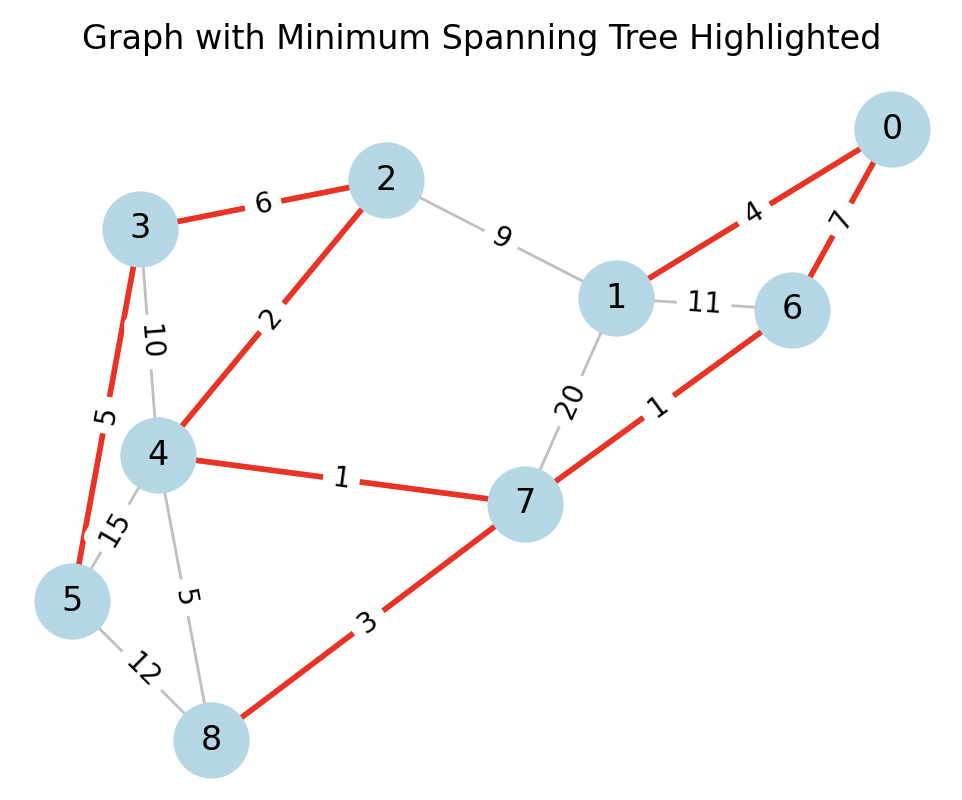
\includegraphics{graph.png}
\subsection{Вхідні та вихідні дані}

\textbf{Вхідні дані} - зважений неорієнтований граф. В нашому випадку представлений списком суміжності або матрицею суміжності.\\
\textbf{Вихідні дані} - мінімальне кістякове дерево графа.

\subsection{Алгоритм}
\begin{verbatim}	
	function Boruvka(G):
	input: graph G with weights on edges
	output: minimum spanning tree T
	for each vertex v in G:
		create a set {v}
	T = empty graph with the same vertices as G
	while T has fewer than n-1 edges:
		for each set S in the set of sets:
			find the edge e with the smallest weight that connects S with a vertex outside S
	if e does not create a cycle in T:
		add e to T
	unite the sets that e connect
	
	return T
\end{verbatim}
\subsection{Оцінки складності}
Часова складність: \(O(E\log V)\), де \(E\) - кількість ребер, а \(V\) - кількість вершин. \\
Просторова складність: \(O(V+E)\).

\section{Короткий опис програмної реалізації}

Наш алгоритм працює за принципом створення 
графу і згодом пошук мінімального кістякового дерева.\\
Спочатку ми зробили реалізацію неорієнтованого графу з вершинами та ребрами. Кожна вершина має список суміжних вершин, створений, щоб при додаванні ребра перевіряти на наявність ребра, який вже з'єднує ці вершини. Кожне ребро має дві кінцеві вершини та вагу. Оскільки це неорієнтований граф, вони просто названі Vertex1 i Vertex2. \\

В об’єкті Graph ми зробили список, який містить в собі вершини та ребра. Він має усі методи роботи з графом, наприклад такі, як додавання та видалення вершин, ребер, а також перевірку суміжності двох вершин. Також реалізовані методи для отримання списку суміжності вершини та перетворення графу в матрицю суміжності, також можливий перехід від списку до матриці та навпаки.\\

Обрано такі рішення та типи даних:
Реалізовано власні класи Vertex та Edge для представлення вершин та ребер відповідно. Кожен клас містить необхідні поля та конструктори.
Vertex: Репрезентує вершину в графі. Кожна вершина має ім'я та список сусідів.
Edge: Репрезентує ребро в неорієнтоаному графі. Кожне ребро з'єднує дві вершини і має вагу.
Для представлення графу використано клас Graph, який містить список вершин та ребер. Використання списків дозволяє легко маніпулювати вершинами та ребрами графу.\\

В ціломую код використовує клас List із .NET Framework для зберігання вершин і ребер, що забезпечує функціональність динамічного масиву та швидкий амортизований час доступу і додавання O(1), звичайно ми також могли зробити і через Set, адже вершини та ребра графа лежать в множинах, але ми вибрали працювати зі списками, бо вони мають більший та кращий як для нас функціонал в C\#. У гіршому випадку метод Remove зі списку має час виконання O(n), але це прийнятно для використання за призначенням.\\

Також були створені два методи перший з яких це \textbf {AdjacencyList} він повертає словник списків сусідів, де ключ це вершина, а значення це список, що містить пари (Сусідня вершина, Вага ребра до неї). Це представлення дозволяє ефективну ітерацію сусідів вершини з часом виконання O(deg (v)) для вершини ступеня deg(v). Загальна складність буде $O(\sum deg(v))$, тобто сума степенів вершин.\\

Другий Метод \textbf{AdjacencyMatrix} він повертає двовимірний масив, який представляє графік як матрицю суміжності. Це представлення дає змогу ефективно знаходити ваги ребер між вершинами, а час виконання для доступу до одного запису становить $O(1)$. Але час виконання для створення матриці суміжності дорівнює $O(n^{2})$, де n - кількість вершин.\\
Загалом, код забезпечує гнучку та ефективну реалізацію структур даних графів.


\section{Посилання на GitHub-репозиторій}
\url{https://github.com/Oleksii-Stepanyk/DM_Project}

\section{Експериментальна частина}
\subsection{Схема експерименту та обрані параметри}
Для проведення чисельних експериментів, нам потрібно визначитись з параметрами, а саме зі щільністю та розмірністю графа.
Оскільки наш алгоритм шукає мінімальне кістякове дерево графу, найкраще буде перевірити його в алгоритмічно складніших умовах, коли ребер багато і степені вершин $\approx$ хоча б половині кількості вершин.\\

Ми обрали 5 щільностей з кроком 12\% від 52\% до 100\%, а саме: \textbf{52\%, 64\%, 76\%, 88\%, 100\%} \\
Для розмірності обрали 10 діапазонів від 20 до 200 з кроком 18: \textbf{20-38, 38-56, 56-74, 74-92, 92-110, 100-128, 128-146, 146-164, 164-182, 182-200}.\\

Для кожної пари розмір-щільність ми провели по 20 експериментальних виконань алгоритм як для матриці суміжності, так і для списку суміжності. Цього повинно бути \textbf{достатньо}, щоб більш точно визначити середній час виконання для цих пар і складність алгоритму в загальному. Схему виконання експерименту детально можна глянути у файлі \textbf{"Program.cs"}, але якщо коротко, то:
\begin{itemize}
	\item Згенерувати граф
	\item Перевести в матрицю або список суміжності
	\item Знайти кістякове дерево
	\item Записати час виконання в список
	\item Зробити так 20 разів для матриць і для списків
	\item Знайти середнє значення виконання для пари (Розмір, щільність)
	\item Вивести в консоль, щоб потім зручно переписати в табличку.
\end{itemize}

\subsection{Результати експериментів}

Дані таблиці та графіки відображають середній час виконання для кожної пари (розмір, щільність).
Таблиці та графіки є розподілені за розмірністю графів. Зліва знаходяться таблиці, що описують час виконання алгоритму з допомогою списків суміжності, справа за допомогою матриць суміжності. \\
Графіки впорядковані з верху в низ, з ліва на право за розмірністю від меншої до більшої \\

\begin{table}[htbp]
\begin{minipage}[b]{0.5\linewidth}
\begin{tabular}{|c|c|c|}
\hline
Розмір & Щільність & Середній час\\
\hline
20-38 & 52\% & 1.1014 \\
20-38 & 64\% & 1.0392 \\
20-38 & 76\% & 1.2010 \\
20-38 & 88\% & 1.4879 \\
20-38 & 100\% & 1.1045 \\
\hline
\end{tabular}
\caption{Списки суміжності}
\end{minipage}
\begin{minipage}[b]{0.5\linewidth}
\begin{tabular}{|c|c|c|}
\hline
Розмір & Щільність & Середній час\\
\hline
20-38 & 52\% & 0.7674 \\
20-38 & 64\% & 0.7117 \\
20-38 & 76\% & 1.3897 \\
20-38 & 88\% & 1.4471 \\
20-38 & 100\% & 1.2910 \\
\hline
\end{tabular}
\caption{Матриці суміжності}
\end{minipage}
\end{table}
\begin{table}[htbp]
\begin{minipage}[b]{0.5\linewidth}
\begin{tabular}{|c|c|c|}
\hline
Розмір & Щільність & Середній час\\
\hline
38-56 & 52\% & 2.0117 \\
38-56 & 64\% & 2.7527 \\
38-56 & 76\% & 2.5989 \\
38-56 & 88\% & 2.9797 \\
38-56 & 100\% & 4.0538 \\
\hline
\end{tabular}
\caption{Списки суміжності}
\end{minipage}
\begin{minipage}[b]{0.5\linewidth}
\begin{tabular}{|c|c|c|}
\hline
Розмір & Щільність & Середній час\\
\hline
38-56 & 52\% & 1.9418 \\
38-56 & 64\% & 2.5784 \\
38-56 & 76\% & 2.7865 \\
38-56 & 88\% & 3.2306 \\
38-56 & 100\% & 3.7311 \\
\hline
\end{tabular}
\caption{Матриці суміжності}
\end{minipage}
\end{table}
\begin{table}[htbp]
\begin{minipage}[b]{0.5\linewidth}
\begin{tabular}{|c|c|c|}
\hline
Розмір & Щільність & Середній час\\
\hline
56-74 & 52\% & 4.9268 \\
56-74 & 64\% & 6.3517 \\
56-74 & 76\% & 6.9198 \\
56-74 & 88\% & 7.4413 \\
56-74 & 100\% & 11.0429 \\
\hline
\end{tabular}
\caption{Списки суміжності}
\end{minipage}
\begin{minipage}[b]{0.5\linewidth}
\begin{tabular}{|c|c|c|}
\hline
Розмір & Щільність & Середній час\\
\hline
56-74 & 52\% & 4.9103 \\
56-74 & 64\% & 5.9150 \\
56-74 & 76\% & 6.6013 \\
56-74 & 88\% & 8.9268 \\
56-74 & 100\% & 9.6470 \\
\hline
\end{tabular}
\caption{Матриці суміжності}
\end{minipage}
\end{table}
\begin{table}[htbp]
\begin{minipage}[b]{0.5\linewidth}
\begin{tabular}{|c|c|c|}
\hline
Розмір & Щільність & Середній час\\
\hline
74-92 & 52\% & 10.8591 \\
74-92 & 64\% & 11.2733 \\
74-92 & 76\% & 16.2188 \\
74-92 & 88\% & 16.0359 \\
74-92 & 100\% & 17.6935 \\
\hline
\end{tabular}
\caption{Списки суміжності}
\end{minipage}
\begin{minipage}[b]{0.5\linewidth}
\begin{tabular}{|c|c|c|}
\hline
Розмір & Щільність & Середній час\\
\hline
74-92 & 52\% & 10.5447 \\
74-92 & 64\% & 11.5420 \\
74-92 & 76\% & 14.6333 \\
74-92 & 88\% & 17.0027 \\
74-92 & 100\% & 20.4048 \\
\hline
\end{tabular}
\caption{Матриці суміжності}
\end{minipage}
\end{table}
\begin{table}[htbp]
\begin{minipage}[b]{0.51\linewidth}
\begin{tabular}{|c|c|c|}
\hline
Розмір & Щільність & Середній час\\
\hline
92-110 & 52\% & 17.2447 \\
92-110 & 64\% & 21.0637 \\
92-110 & 76\% & 24.5627 \\
92-110 & 88\% & 27.2734 \\
92-110 & 100\% & 32.5348 \\
\hline
\end{tabular}
\caption{Списки суміжності}
\end{minipage}
\begin{minipage}[b]{0.51\linewidth}
\begin{tabular}{|c|c|c|}
\hline
Розмір & Щільність & Середній час\\
\hline
92-110 & 52\% & 15.5890 \\
92-110 & 64\% & 20.9771 \\
92-110 & 76\% & 23.5322 \\
92-110 & 88\% & 26.5830 \\
92-110 & 100\% & 31.3560 \\
\hline
\end{tabular}
\caption{Матриці суміжності}
\end{minipage}
\end{table}
\begin{table}[htbp]
\begin{minipage}[b]{0.51\linewidth}
\begin{tabular}{|c|c|c|}
\hline
Розмір & Щільність & Середній час\\
\hline
110-128 & 52\% & 26.8040 \\
110-128 & 64\% & 36.9913 \\
110-128 & 76\% & 42.7980 \\
110-128 & 88\% & 48.7638 \\
110-128 & 100\% & 54.4259 \\
\hline
\end{tabular}
\caption{Списки суміжності}
\end{minipage}
\begin{minipage}[b]{0.51\linewidth}
\begin{tabular}{|c|c|c|}
\hline
Розмір & Щільність & Середній час\\
\hline
110-128 & 52\% & 28.3031 \\
110-128 & 64\% & 37.8035 \\
110-128 & 76\% & 39.8457 \\
110-128 & 88\% & 49.8018 \\
110-128 & 100\% & 49.2711 \\
\hline
\end{tabular}
\caption{Матриці суміжності}
\end{minipage}
\end{table}
\begin{table}[htbp]
\begin{minipage}[b]{0.51\linewidth}
\begin{tabular}{|c|c|c|}
\hline
Розмір & Щільність & Середній час\\
\hline
128-146 & 52\% & 39.9332 \\
128-146 & 64\% &50.7484 \\
128-146 & 76\% & 59.4270 \\
128-146 & 88\% & 64.8131 \\
128-146 & 100\% & 77.5845 \\
\hline
\end{tabular}
\caption{Списки суміжності}
\end{minipage}
\begin{minipage}[b]{0.51\linewidth}
\begin{tabular}{|c|c|c|}
\hline
Розмір & Щільність & Середній час\\
\hline
128-146 & 52\% & 45.9768 \\
128-146 & 64\% &48.7960 \\
128-146 & 76\% &58.7248 \\
128-146 & 88\% & 66.2854 \\
128-146 & 100\% & 81.5494 \\
\hline
\end{tabular}
\caption{Матриці суміжності}
\end{minipage}
\end{table}
\begin{table}[htbp]
\begin{minipage}[b]{0.51\linewidth}
\begin{tabular}{|c|c|c|}
\hline
Розмір & Щільність & Середній час\\
\hline
146-164 & 52\% & 60.5990 \\
146-164 & 64\% & 73.0276 \\
146-164 & 76\% & 91.4424 \\
146-164 & 88\% & 96.5072 \\
146-164 & 100\% & 123.2196 \\
\hline
\end{tabular}
\caption{Списки суміжності}
\end{minipage}
\begin{minipage}[b]{0.51\linewidth}
\begin{tabular}{|c|c|c|}
\hline
Розмір & Щільність & Середній час\\
\hline
146-164 & 52\% & 62.6559 \\
146-164 & 64\% & 72.2091 \\
146-164 & 76\% & 86.9954 \\
146-164 & 88\% & 109.8839 \\
146-164 & 100\% & 116.5637 \\
\hline
\end{tabular}
\caption{Матриці суміжності}
\end{minipage}
\end{table}
\begin{table}[htbp]
\begin{minipage}[b]{0.51\linewidth}
\begin{tabular}{|c|c|c|}
\hline
Розмір & Щільність & Середній час\\
\hline
164-182 & 52\% & 82.5564 \\
164-182  & 64\% & 97.9248 \\
164-182  & 76\% & 116.8207 \\
164-182  & 88\% & 136.7831 \\
164-182  & 100\% & 157.1514 \\
\hline
\end{tabular}
\caption{Списки суміжності}
\end{minipage}
\begin{minipage}[b]{0.51\linewidth}
\begin{tabular}{|c|c|c|}
\hline
Розмір & Щільність & Середній час\\
\hline
164-182  & 52\% & 88.2309 \\
164-182  & 64\% & 110.0523 \\
164-182  & 76\% & 122.3699 \\
164-182  & 88\% & 135.3454 \\
164-182  & 100\% & 171.1403 \\
\hline
\end{tabular}
\caption{Матриці суміжності}
\end{minipage}	
\end{table}
\begin{table}[htbp]
\begin{minipage}[b]{0.51\linewidth}
\begin{tabular}{|c|c|c|}
\hline
Розмір & Щільність & Середній час\\
\hline
182-200 & 52\% & 112.8464 \\
182-200  & 64\% & 133.5016 \\
182-200  & 76\% & 155.0467 \\
182-200  & 88\% & 212.4126 \\
182-200  & 100\% & 209.2285 \\
\hline
\end{tabular}
\caption{Списки суміжності}
\end{minipage}
\begin{minipage}[b]{0.51\linewidth}
\begin{tabular}{|c|c|c|}
\hline
Розмір & Щільність & Середній час\\
\hline
182-200  & 52\% & 116.9804 \\
182-200  & 64\% & 135.0831 \\
182-200  & 76\% & 165.0716 \\
182-200  & 88\% & 200.4955 \\
182-200  & 100\% & 216.8950 \\
\hline
\end{tabular}
\caption{Матриці суміжності}
\end{minipage}
\end{table}
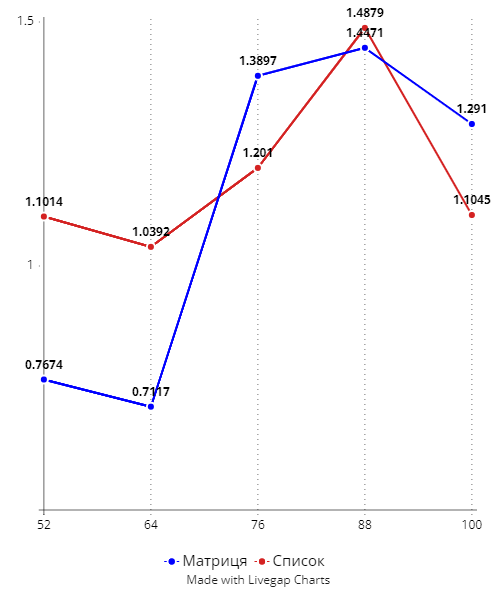
\includegraphics[width=0.5\linewidth]{20-38.png}
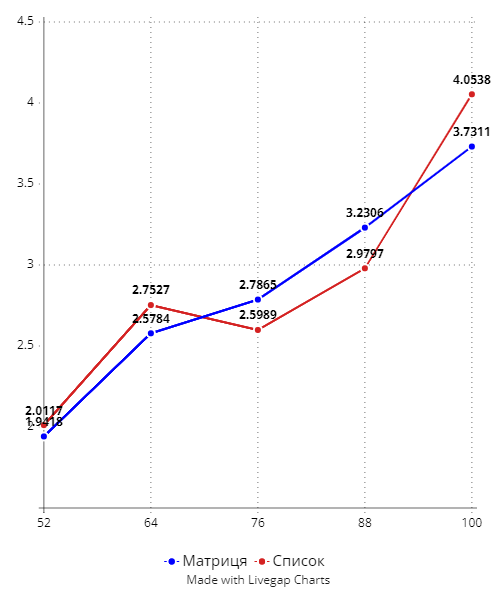
\includegraphics[width=0.5\linewidth]{38-56.png}
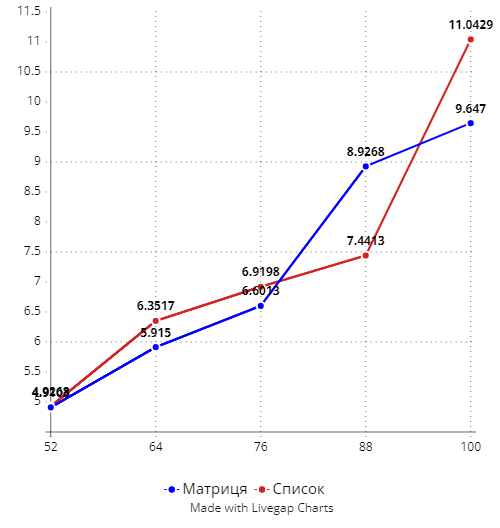
\includegraphics[width=0.5\linewidth]{56-74.png}
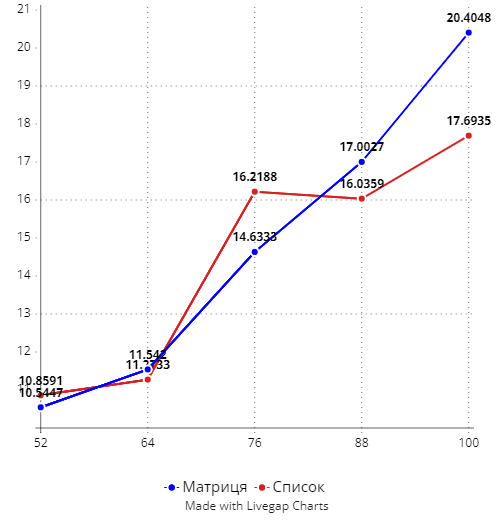
\includegraphics[width=0.5\linewidth]{74-92.png}
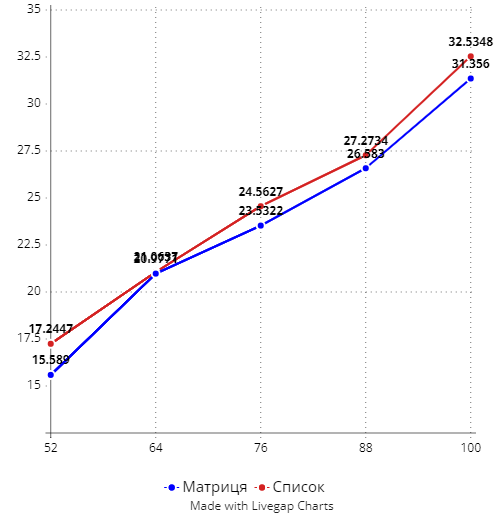
\includegraphics[width=0.5\linewidth]{92-110.png}
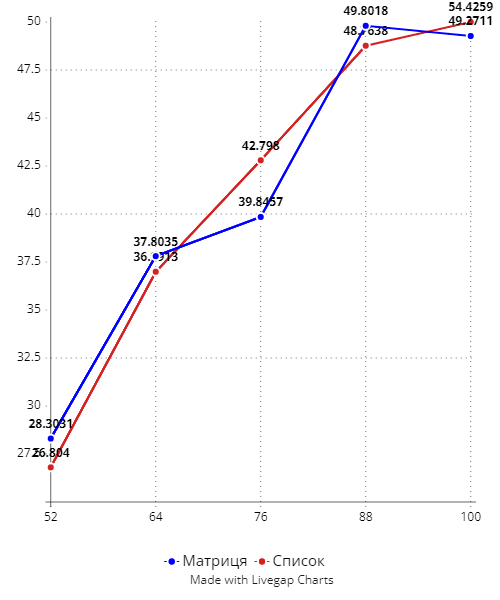
\includegraphics[width=0.5\linewidth]{110-128.png}
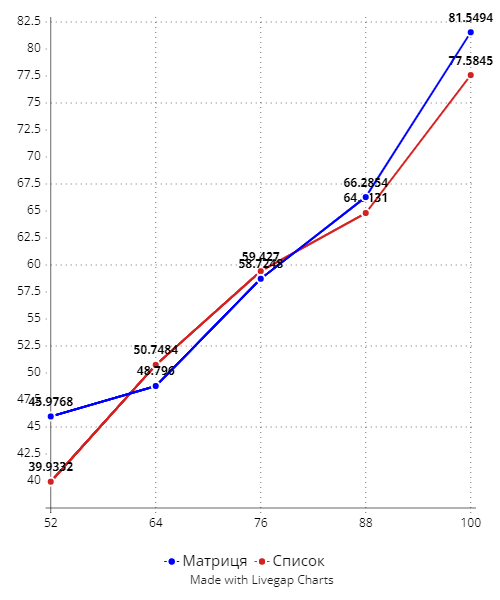
\includegraphics[width=0.5\linewidth]{128-146.png}
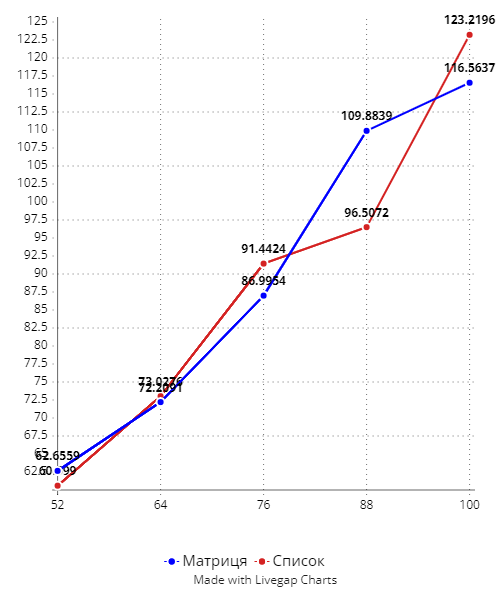
\includegraphics[width=0.5\linewidth]{146-164.png}
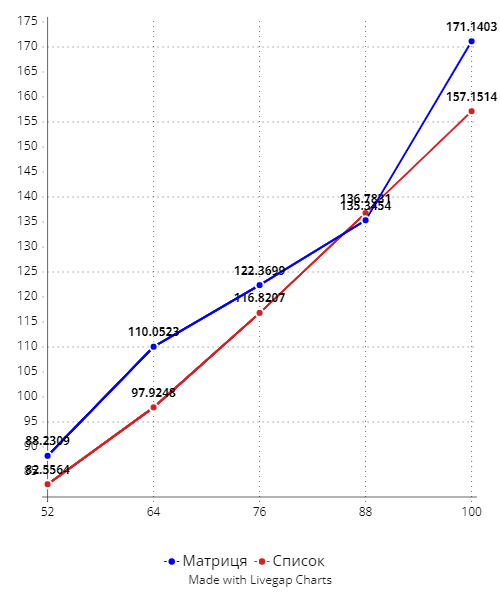
\includegraphics[width=0.5\linewidth]{164-182.png}
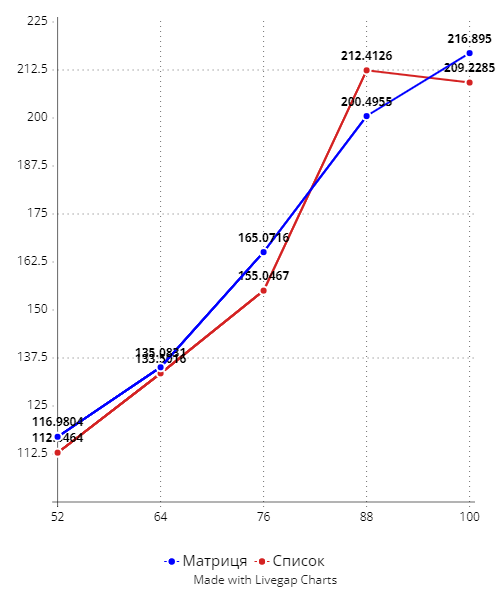
\includegraphics[width=0.5\linewidth]{182-200.png}

\subsection{Аналіз результатів}
Найперше, що можна побачити в, переоформлених в таблиці та графіки, результатах, це те, як росте час виконання в залежності від щільності графа. Чим щільніший граф, тим більше він містить ребер, які в свою чергу є основним показником часової складності алгоритму.\\
Наступна закономірність, яка помітна це те, що час пошуку мінімального кістякового дерева для графу певної розмірності зі щільністю 95-100\% $\approx$ часу пошуку мінімального кістякового дерева для графу більшої розмірності зі щільністю 50-55\%. Це можна пояснити тим, що якщо взяти кількість ребер графу з n вершин при 100\%-ій щільності і кількість ребер з n+20 50\%-ій щільності, вийде приблизно та сама кількість ребер. Саме через це час виконання майже схожий, невелика похибка якраз таки виражена в різниці кількості вершин, адже складність алгоритму від вершин зростає зі швидкістю $\log_{2}(v)$.\\
Зрештою це також працюватиме і в просторовій складності, адже умовно різниця між |E|+|V| та |E|+|V+20| лише 20 бітів\textit{(вершина звісно займатиме більше, але це не дуже суттєво, навіть для 200 вершин)}.\\
Останнє, на що хочеться вказати, це те, що якщо з'єднати усі графіки середнього виконання алгоритму, то вийде графік, дуже схожий\textit{(або навіть він самий)} на $\frac{n*(n-1)}{2}*log(n)$, що є в свою чергу $|E|*log|V|$. Ми можемо так з'єднати, адже вже раніше показали, що в більшому графі меншої щільності буде схожа кількість ребер при меншому графі більшої щільності. Завдяки цьому, ми можемо стверджувати, що практична часова та просторова складність відповідає теоретичній та на певній фіксованій щільності буде зростати експоненційно.\\

Дуже неприємним є графік для зовсім малих графів (20-38 вершин), там по якійсь причині з ростом щільності час нерівномірно зростає та спадає. Складно дати відповідь з чим це зумовлено, можливо через те, що відмінність у 1-2 вершини суттєво міняє час виконання.

Вплив представлення на алгоритм: З проаналізованих результатів можемо побачити, що представлення мінімально впливає на алгоритм.
В середньому на менших графах матриці суміжності працюють краще, ніж списки. А ось на більших вийшло дещо навпаки.\\
Але в цілому обидва способи представлення графа показують однаковий результат з чого випливає те, що алгоритму не сильно важливо те, яким способом представляти алгоритм, адже він в будь-якому випадку (як мінімум у нашій імплементації) працює з самими ребрами.

\section{Особистий внесок}
\subsection*{Кирило Шихальов}
Повністю написав формальний опис алгоритму, від 1.1 до 1.4 включно. Написав короткий опис до програмної реалізації, посилання на репозиторій та висновки. Все було написано латексом.
\subsection*{Олексій Степаник}
Написав 99.1\% коду, що включає в себе всі класи, алгоритм, генерації вершин та графів та сам експеримент. Написав експериментальну частину, створив для неї графіки та написав таблиці, також написав висновки.
\section{Висновки}

Отже, ми проаналізували вхідні та вихідні дані, які приймає та повертає алгоритм.\\
В першу чергу експеримент проєкту показує, що використання певного представлення графу майже не впливає на час виконання алгоритму. Єдині суттєві відмінності можуть виникнути в просторовій складності, якщо неоптимально зберігати та конвертувати необхідні алгоритму значення. \\

Наступне, фактична складність алгоритму є такою ж, як і теоретична. З цього випливає, що той, хто оцінював алгоритм, правильного його оцінив і також завдяки цьому ми тепер можемо на практиці використовувати теоретичну оцінку складності.\\

Цей проєкт навчив нас реалізовувати алгоритми самому в коді, досліджувати їх більш обширно так, щоб можна було проаналізувати результати виконання та дізнатись чи дійсно теоретична складність відповідає дійсності. Також за допомогою цих же результатів ми змогли побачити з яким представленням графу алгоритм працює краще.\\

\section{Основні джерела}
https://en.wikipedia.org/wiki/Borůvka\%27s\_algorithm: \\
Література для ознайомлення з алгоритмом. \textbf{\textit{(Посилання не відформатовано через проблему з символом ů)}}\\
\url{https://medium.com/@arst-dev/algorithms-in-c-borůvkas-algorithm-c82239ef3f0c}: \\
Реалізація алгоритму на C\#, яка була почастинно проаналізована і використана як точка відштовху для кращого розуміння та написання алгоритму.\\
\url{https://chat.openai.com}:\\
 AI Помічник, який допоміг з розумінням розмітки LaTeX'у, допомагав знаходити потрібні packages для LaTeX та час від часу допомагав фіксити код в моментах, коли помилка була непомітна людському оку, АЛЕ не писав за нас ні код, ні текст в LaTeX.\\
\url{https://blog.writefull.com/the-100-most-frequent-latex-commands/}:\\
 Оскільки GPT швидше шукає потрібний синтаксис, цей сайт користі не приніс, але має право бути тут.
\url{https://charts.livegap.com/?lan=en}: \\
Сайт з допомогою якого було створено лінійні графіки
\end{document}
